%! TeX program = xelatex

\documentclass[12pt,a4paper]{report}
\usepackage{fontspec}
\IfFontExistsTF{Calibri}{
  \setmainfont{Calibri}
}{
  \setmainfont{Carlito}
}
\usepackage[indonesian]{babel}
\usepackage[none]{hyphenat}
\sloppy
\usepackage[
  left=4cm,
  right=3cm,
  top=3cm,
  bottom=3cm
]{geometry}
\usepackage{setspace}
\doublespacing
\setlength{\parskip}{0pt}
\setlength{\parindent}{0.75cm}
\usepackage{titlesec}
\usepackage{graphicx}
\usepackage{float}

\titleformat{\chapter}[display]
  {\normalfont\bfseries\fontsize{12pt}{14.4pt}\selectfont\centering}
  {BAB \Roman{chapter}}
  {0pt}
  {}

\titlespacing*{\chapter}
  {0pt}
  {0pt}
  {\baselineskip}

\titleformat{\section}[hang]
  {\normalfont\bfseries\fontsize{12pt}{14.4pt}\selectfont}
  {\thesection}
  {1em}
  {}

\titlespacing*{\section}
  {0pt}
  {\baselineskip}
  {0.5\baselineskip}
\usepackage{enumitem}
\usepackage[hidelinks]{hyperref}


\widowpenalty=10000
\clubpenalty=10000
\displaywidowpenalty=10000

\setlist[enumerate]{
  itemsep=0pt,
  topsep=0pt
}
\setcounter{secnumdepth}{3}
\setcounter{tocdepth}{3}

% =========================================================
% DOCUMENT
% =========================================================
\begin{document}

\pagenumbering{roman}
\tableofcontents
\clearpage
\pagenumbering{arabic}

\chapter{PENDAHULUAN}

\section{Latar Belakang}

Restoran Nasi Padang merupakan salah satu jenis rumah makan yang mudah ditemukan di Indonesia. Salah satu karakteristiknya adalah tersedianya berbagai jenis lauk yang dapat dipilih pelanggan, seperti rendang, perkedel, telur dadar, sayur nangka, daun singkong, telur kari, dan sambal. Pada pelayanan konvensional, pelanggan menyampaikan lauk yang diinginkan kepada staf, kemudian staf mengambilkan lauk tersebut untuk pelanggan. Setelah selesai makan, pelanggan menghampiri staf pada bagian pembayaran dan menyebutkan satu per satu jenis serta jumlah lauk yang telah dikonsumsi berdasarkan ingatan pelanggan. Staf kemudian menghitung total harga dari lauk yang disebutkan dan menyampaikan jumlah yang harus dibayarkan kepada pelanggan.

Dalam kondisi jumlah pelanggan yang tinggi, proses pengambilan lauk tersebut dapat menyebabkan pelanggan harus menunggu ketersediaan staf sebelum dapat dilayani. Pada saat yang sama, staf perlu membagi perhatian antara melayani pelanggan \textit{dine-in} dan menangani pesanan lain, termasuk pesanan \textit{take-away}. Kondisi ini dapat menimbulkan antrean pada proses pelayanan dan mengurangi efisiensi kerja staf.

Untuk mengatasi permasalahan tersebut, penelitian ini mengusulkan alternatif pelayanan berupa \textit{self-service} untuk pelanggan \textit{dine-in}. Pada mekanisme ini, pelanggan dapat mengambil dan memilih sendiri lauk yang diinginkan dari lauk yang tersedia, kemudian membawa piring yang telah dipilih ke proses \textit{checkout}. Dengan demikian, pelanggan tidak perlu menunggu staf untuk mengambilkan lauk satu per satu. Penerapan mekanisme \textit{self-service} juga memungkinkan staf untuk mengurangi aktivitas pelayanan pengambilan lauk \textit{dine-in} sehingga dapat lebih berfokus pada pelayanan lain, khususnya pemenuhan pesanan \textit{take-away}.

Agar mekanisme tersebut dapat diterapkan tanpa mengharuskan staf memeriksa
kembali lauk yang dipilih pelanggan secara \textit{self-service}, diperlukan
suatu sistem yang mampu mengenali isi piring secara otomatis. Kebutuhan
tersebut merupakan salah satu permasalahan yang dapat ditangani menggunakan
\textit{Computer Vision}. Pemanfaatan \textit{Computer Vision} dalam analisis
makanan telah mencakup berbagai tugas seperti pengenalan, deteksi, dan
segmentasi makanan \cite{min2019}.

Dalam beberapa kasus lauk yang terdapat pada satu piring, pengenalan kelas
saja belum cukup karena sistem juga perlu membedakan setiap lauk sebagai
objek yang terpisah untuk menghitung jumlahnya. Oleh karena itu, penelitian
ini menggunakan \textit{instance segmentation}. \textit{Instance segmentation}
menghasilkan informasi kelas sekaligus \textit{mask} untuk setiap instans
objek sehingga beberapa objek dari kelas yang sama tetap dapat
direpresentasikan secara terpisah \cite{he2017maskrcnn}.

Kemampuan tersebut sesuai dengan karakteristik objek makanan yang dapat
memiliki bentuk tidak beraturan dan saling menutupi serta dengan kebutuhan
sistem \textit{checkout} untuk menghitung setiap instans secara individual
\cite{guo2023,nguyen2022sibnet,nguyen2023foodmask}. Total pembayaran pada
sistem yang dirancang ditentukan berdasarkan jenis dan jumlah lauk, bukan
berdasarkan luas area lauk pada citra.

Salah satu model yang digunakan dalam pengembangan \textit{object detection} adalah YOLO (\textit{You Only Look Once}). YOLO dirancang untuk mendeteksi objek dalam citra dengan melakukan lokalisasi dan klasifikasi dalam satu proses inferensi. Seiring perkembangannya, keluarga YOLO tidak hanya digunakan untuk \textit{object detection}, tetapi juga mendukung beberapa tugas \textit{Computer Vision} lainnya, termasuk \textit{image classification} dan \textit{instance segmentation} \cite{khanam2024}.

YOLO11 merupakan salah satu versi dari keluarga YOLO yang dikembangkan dengan peningkatan pada arsitektur dan efisiensi model. YOLO11 mendukung beberapa tugas \textit{Computer Vision}, termasuk \textit{instance segmentation}. Untuk tugas tersebut, digunakan varian YOLO11-seg yang menghasilkan informasi kelas dan \textit{pixel mask} untuk setiap objek yang terdeteksi \cite{khanam2024,qiu2025}. Output tersebut memungkinkan sistem untuk menentukan batas setiap lauk dan membedakan beberapa lauk sebagai instans yang terpisah sehingga jumlahnya dapat dihitung secara otomatis. Berdasarkan kebutuhan tersebut, YOLO11-seg digunakan sebagai model utama dalam penelitian ini.

Berdasarkan uraian tersebut, penelitian ini merancang \textit{proof-of-concept} sistem \textit{checkout} otomatis yang menyediakan opsi \textit{self-service} bagi pelanggan \textit{dine-in} restoran Nasi Padang. Pelanggan dapat mengambil lauk secara mandiri, kemudian sistem menggunakan YOLO11-seg untuk mendeteksi, melakukan \textit{instance segmentation}, dan menghitung setiap instans lauk pada piring. Hasil tersebut selanjutnya digunakan untuk menghitung total pembayaran berdasarkan harga tetap setiap kelas lauk. Penelitian ini dibatasi pada sembilan kelas, yaitu nasi, rendang, ayam goreng, perkedel, sayur nangka, daun singkong, telur dadar, telur kari, dan sambal.

Berdasarkan latar belakang tersebut, penelitian ini mengusulkan judul ``Deteksi Lauk Nasi Padang untuk Sistem \textit{Checkout} Otomatis dengan \textit{Instance Segmentation} Menggunakan YOLO11''.


\section{Rumusan Rancangan}

Berdasarkan latar belakang yang telah diuraikan, penelitian ini berfokus pada perancangan sistem \textit{checkout} otomatis yang memanfaatkan \textit{instance segmentation} untuk mengenali dan menghitung lauk Nasi Padang. Rumusan rancangan dalam penelitian ini adalah sebagai berikut:

\begin{enumerate}
    \item Bagaimana merancang dan melatih model \textit{instance segmentation} menggunakan arsitektur YOLO11-seg agar mampu mendeteksi dan melakukan segmentasi terhadap sembilan kelas lauk Nasi Padang serta menghasilkan prediksi setiap instans objek secara individual?

    \item Bagaimana mengevaluasi performa YOLO11-seg dalam mendeteksi, melakukan segmentasi, dan menghitung instans lauk Nasi Padang berdasarkan hasil pengujian model?

    \item Bagaimana merancang alur integrasi hasil deteksi dan \textit{instance counting} dari YOLO11-seg dengan sistem penetapan harga berbasis \textit{fixed price} untuk menghasilkan total tagihan secara otomatis?
\end{enumerate}


\section{Komponen Perancangan}

Sistem \textit{checkout} otomatis yang dirancang dalam penelitian ini terdiri atas tiga komponen utama yang saling terhubung dalam proses \textit{checkout}, yaitu kamera, model YOLO11-seg, dan program kalkulasi harga.

\begin{enumerate}
    \item \textbf{Kamera}

    Kamera berfungsi sebagai komponen akuisisi citra pada proses \textit{checkout}. Kamera digunakan untuk memperoleh citra piring yang telah berisi lauk pilihan pelanggan. Citra tersebut kemudian digunakan sebagai masukan bagi model YOLO11-seg untuk melakukan proses pengenalan lauk.

    \item \textbf{Model YOLO11-seg}

    YOLO11-seg merupakan komponen utama dalam pemrosesan \textit{Computer Vision} pada sistem. Model ini digunakan untuk mendeteksi dan melakukan \textit{instance segmentation} terhadap lauk yang terdapat pada citra piring. Dari hasil prediksi tersebut, sistem memperoleh kelas dan setiap instans lauk yang terdeteksi sehingga jumlah lauk dari masing-masing kelas dapat dihitung.

    \item \textbf{Program Kalkulasi Harga}

    Program kalkulasi harga berfungsi mengolah hasil pengenalan dan penghitungan instans dari YOLO11-seg menjadi total pembayaran. Program menggunakan harga tetap untuk setiap kelas lauk, kemudian menghitung total harga berdasarkan jenis dan jumlah instans lauk yang terdeteksi.
\end{enumerate}


\section{Spesifikasi Perancangan}

Spesifikasi perancangan sistem \textit{checkout} otomatis lauk Nasi Padang dalam penelitian ini terdiri atas tiga modul utama yang saling terhubung, yaitu modul akuisisi citra, modul pengenalan lauk menggunakan YOLO11-seg, dan modul kalkulasi harga.

\begin{enumerate}
    \item \textbf{Modul Akuisisi Citra}

    Modul akuisisi citra berfungsi memperoleh citra piring yang berisi lauk pilihan pelanggan menggunakan kamera. Citra yang diperoleh digunakan sebagai masukan bagi model YOLO11-seg. Sistem menggunakan citra digital dua dimensi dalam format RGB sebagai data masukan.

    \item \textbf{Modul Pengenalan Lauk dengan YOLO11-seg}

    Modul pengenalan lauk menggunakan YOLO11-seg untuk mendeteksi dan melakukan \textit{instance segmentation} terhadap lauk yang terdapat pada citra. Model menghasilkan prediksi kelas serta \textit{mask} untuk setiap instans objek yang terdeteksi.

    Hasil prediksi tersebut digunakan untuk menentukan jumlah instans pada setiap kelas. Setiap instans yang terdeteksi dihitung secara individual sehingga beberapa objek dari kelas yang sama tetap dapat dibedakan dan dihitung sebagai objek yang terpisah.

    Pengenalan dibatasi pada sembilan kelas, yaitu nasi, rendang, ayam goreng, perkedel, sayur nangka, daun singkong, telur dadar, telur kari, dan sambal.

    \item \textbf{Modul Kalkulasi Harga}

    Modul kalkulasi harga menggunakan jenis dan jumlah instans lauk yang telah dikenali untuk menentukan total pembayaran. Setiap kelas lauk memiliki harga tetap, kemudian total pembayaran dihitung berdasarkan jumlah instans dari masing-masing kelas. Penentuan harga tidak menggunakan berat, volume, luas \textit{pixel mask}, maupun ukuran porsi.
\end{enumerate}

\section{Kegunaan Rancangan}

Hasil perancangan sistem checkout otomatis ini diharapkan dapat memberikan kegunaan secara operasional maupun teknis dan akademis. Secara keseluruhan, rancangan ini menjadi \textit{proof-of-concept} penerapan \textit{self-service} dan otomatisasi proses \textit{checkout} pada restoran Nasi Padang dengan memanfaatkan \textit{Computer Vision}.

Secara operasional, sistem yang dirancang dapat digunakan sebagai alternatif mekanisme \textit{checkout} bagi pelanggan \textit{dine-in}. Sistem memanfaatkan YOLO11-seg untuk mengenali dan menghitung lauk yang terdapat pada piring, kemudian hasil tersebut digunakan untuk menentukan total pembayaran secara otomatis. Penerapan mekanisme ini diharapkan dapat mengurangi ketergantungan terhadap staf dalam proses pencatatan lauk pelanggan \textit{dine-in} serta memberikan alternatif pelayanan yang lebih mandiri.

Secara teknis dan akademis, penelitian ini memberikan penerapan dan evaluasi YOLO11-seg pada \textit{use-case} pengenalan dan penghitungan lauk Nasi Padang yang memiliki karakteristik objek dan kelas yang spesifik. Hasil evaluasi dapat memberikan gambaran mengenai kemampuan model dalam mendeteksi, melakukan \textit{instance segmentation}, dan menghitung setiap instans lauk. Dengan demikian, penelitian ini dapat menjadi referensi awal untuk penerapan \textit{Computer Vision} berbasis \textit{instance segmentation} pada sistem \textit{checkout} makanan dengan jenis dan jumlah objek sebagai dasar penentuan harga.

\section{Rancangan yang Sudah Dibuat}

Beberapa penelitian sebelumnya telah mengembangkan sistem dan metode yang berkaitan dengan pengenalan makanan, \textit{instance segmentation}, penghitungan instans, dan sistem \textit{checkout} otomatis. Beberapa rancangan yang relevan dengan penelitian ini adalah sebagai berikut:

\begin{enumerate}
    \item Perancangan yang berjudul ``Grab, Pay and Eat: Semantic Food Detection for Smart Restaurants'' oleh Aguilar et al. mengembangkan metode \textit{Semantic Food Detection} untuk menganalisis makanan pada nampan di lingkungan restoran. Metode tersebut menggabungkan proses lokalisasi, pengenalan, deteksi, dan segmentasi makanan untuk mendukung penerapan \textit{automatic billing} pada restoran \textit{self-service}. Penelitian tersebut memperoleh nilai F-measure sekitar 90\% pada dataset UNIMIB2016 \cite{aguilar2017}.

    \item Perancangan yang berjudul ``A Framework of Visual Checkout System Using Convolutional Neural Networks for Bento Buffet'' oleh Wu et al. mengembangkan sistem \textit{visual checkout} untuk restoran Bento Buffet menggunakan kamera Kinect dan CNN. Sistem melakukan pengenalan makanan serta menggunakan informasi kedalaman untuk memperkirakan volume makanan dan harga. Pendekatan pengenalan dua tahap yang digunakan menghasilkan akurasi sebesar 96,3\% pada dataset pengujian \cite{wu2021}.

    \item Perancangan yang berjudul ``A Real-Time Chinese Food Auto Billing System Based on Instance Segmentation'' oleh Guo et al. mengembangkan sistem perhitungan harga makanan Tiongkok secara otomatis menggunakan segmentasi. Sistem mengenali jenis piring berdasarkan bentuk dan ukuran, di mana setiap jenis piring merepresentasikan harga tertentu. Penelitian tersebut juga mengembangkan FoodSyn untuk menghasilkan data sintetis dan memperoleh nilai mIoU lebih dari 95\% pada pengujian yang dilakukan \cite{guo2023}.

    \item Perancangan yang berjudul ``SibNet: Food Instance Counting and Segmentation'' oleh Nguyen et al. mengembangkan jaringan multi-task untuk melakukan penghitungan dan segmentasi instans makanan secara bersamaan. SibNet dirancang untuk menangani karakteristik makanan dengan bentuk yang tidak beraturan serta kondisi objek yang saling menutupi melalui penggunaan \textit{instance seed} dan \textit{sibling relation network} \cite{nguyen2022sibnet}.

    \item Perancangan yang berjudul ``FoodMask: Real-time Food Instance Counting, Segmentation and Recognition'' oleh Nguyen et al. mengembangkan jaringan multi-task untuk melakukan penghitungan, segmentasi, dan pengenalan instans makanan secara bersamaan. FoodMask menghasilkan informasi kategori makanan dan instans pada tingkat piksel serta dirancang untuk melakukan pemrosesan secara \textit{real-time} pada citra yang dapat berisi beberapa jenis makanan \cite{nguyen2023foodmask}.

    \item Perancangan yang berjudul ``Indonesian Street Food Calorie Estimation Using Mask R-CNN and Multiple Linear Regression'' oleh Aditama dan Munir menerapkan Mask R-CNN untuk melakukan \textit{amodal instance segmentation} terhadap enam kelas jajanan Indonesia. Penelitian tersebut secara khusus mengevaluasi kondisi oklusi dan non-oklusi, dengan F1-score sebesar 0,821 pada kondisi oklusi dan 0,994 pada kondisi non-oklusi \cite{aditama2022}.
\end{enumerate}

\chapter{LANDASAN TEORETIK}

\section{Landasan Teori}

Landasan teori pada bagian ini membahas konsep yang digunakan untuk memahami rancangan sistem \textit{checkout} otomatis Nasi Padang. Pembahasan diawali dengan Nasi Padang untuk menjelaskan karakteristik makanan dan bentuk penyajian yang menjadi ruang lingkup penelitian. Selanjutnya, pembahasan mencakup \textit{Computer Vision} dan citra digital, \textit{instance segmentation}, YOLO11-seg, penghitungan instans dan perhitungan total harga, serta evaluasi kinerja model dan sistem. Detail mengenai dataset, konfigurasi pelatihan, perangkat, dan prosedur pengujian dibahas pada Bab III.

\subsection{\textit{Computer Vision} dan Citra Digital}

\textit{Computer Vision} digunakan untuk memperoleh informasi dari citra melalui proses komputasi. Pada analisis makanan, informasi visual dapat dimanfaatkan untuk melakukan pengenalan, deteksi, dan segmentasi objek sehingga jenis serta lokasi makanan pada citra dapat ditentukan \cite{aguilar2017}.

Citra digital berwarna tersusun atas nilai piksel pada beberapa kanal warna. Informasi tersebut menjadi masukan bagi model untuk membentuk representasi fitur yang berkaitan dengan karakteristik visual objek, seperti bentuk, warna, tekstur, dan susunan objek pada citra. Pada sistem yang dirancang, citra piring digunakan sebagai masukan bagi YOLO11-seg untuk mengenali lauk pada tingkat instans.

Karena pengambilan citra pada sistem dilakukan dari posisi tetap di atas piring, area objek dapat diamati dengan perspektif yang relatif konsisten. Pendekatan pengambilan citra dari arah atas juga digunakan pada sistem \textit{visual checkout} makanan untuk memperoleh tampilan objek pada area pengamatan secara konsisten \cite{wu2021}.

\subsection{\textit{Instance Segmentation}}

\textit{Instance segmentation} merupakan tugas \textit{Computer Vision} yang menghasilkan informasi kelas dan wilayah piksel untuk setiap instans objek. Berbeda dengan segmentasi semantik yang memberikan label kelas pada piksel tanpa membedakan objek dari kelas yang sama, \textit{instance segmentation} mempertahankan identitas setiap objek sebagai instans yang terpisah \cite{he2017maskrcnn}.

Pemisahan pada tingkat instans sesuai dengan kebutuhan sistem karena satu piring dapat mengandung lebih dari satu lauk dari kelas yang sama. Setiap objek perlu dipertahankan sebagai instans yang berbeda agar jumlahnya dapat dihitung secara individual. Pemanfaatan segmentasi dan penghitungan pada tingkat instans juga digunakan pada penelitian SibNet dan FoodMask untuk mengenali serta menghitung objek makanan \cite{nguyen2022sibnet,nguyen2023foodmask}.

Kondisi oklusi dapat menjadi tantangan dalam \textit{instance segmentation} karena sebagian area objek dapat tertutup oleh objek lain sehingga informasi visual yang tersedia berkurang \cite{ke2021}. Oleh karena itu, kondisi oklusi dipandang sebagai salah satu faktor yang dapat memengaruhi hasil prediksi model dan bukan sebagai kondisi yang diasumsikan selalu dapat ditangani secara sempurna.

Pada sistem yang dirancang, keluaran \textit{instance segmentation} digunakan untuk memperoleh kelas dan identitas setiap instans lauk. Luas \textit{segmentation mask} tidak digunakan untuk menentukan harga maupun jumlah lauk; jumlah ditentukan berdasarkan banyaknya instans yang dipertahankan sebagai hasil prediksi akhir.

\subsection{YOLO11-seg}

YOLO11-seg merupakan varian YOLO11 yang mendukung tugas \textit{instance segmentation}. Model ini digunakan untuk menghasilkan prediksi lokasi objek, kelas, dan \textit{segmentation mask} dalam satu model sehingga proses klasifikasi lauk dan segmentasi tidak memerlukan dua model yang terpisah \cite{khanam2024,qiu2025}.

\subsubsection*{a. Arsitektur YOLO11-seg}

Secara umum, arsitektur YOLO11 terdiri atas tiga bagian utama, yaitu \textit{backbone}, \textit{neck}, dan \textit{head}. \textit{Backbone} mengekstraksi fitur dari citra masukan, \textit{neck} menggabungkan fitur dari beberapa tingkat resolusi, sedangkan \textit{head} menggunakan fitur tersebut untuk menghasilkan prediksi objek \cite{khanam2024}. Pada YOLO11-seg, bagian keluaran juga mencakup informasi yang diperlukan untuk membentuk segmentasi setiap instans \cite{qiu2025}.

Pada bagian \textit{backbone}, citra diproses melalui lapisan konvolusi dan modul utama seperti C3k2, SPPF (\textit{Spatial Pyramid Pooling--Fast}), dan C2PSA. C3k2 digunakan dalam proses ekstraksi fitur, SPPF memperluas informasi konteks melalui operasi \textit{pooling}, sedangkan C2PSA memberikan mekanisme perhatian terhadap fitur yang diproses \cite{khanam2024,qiu2025}.

Fitur dari \textit{backbone} diteruskan ke bagian \textit{neck}. Bagian ini menggabungkan informasi dari beberapa tingkat resolusi melalui operasi seperti \textit{upsampling} dan \textit{concatenation}. Penggabungan fitur lintas skala memungkinkan informasi spasial dari fitur beresolusi lebih tinggi dipadukan dengan informasi semantik dari fitur yang lebih dalam \cite{khanam2024,qiu2025}.

Hasil dari \textit{neck} kemudian diteruskan ke \textit{head}. Pada YOLO11-seg, bagian deteksi menghasilkan prediksi kelas dan posisi \textit{bounding box}, sedangkan bagian segmentasi menghasilkan informasi \textit{mask} untuk setiap kandidat objek. Salah satu mekanisme yang digunakan adalah pembentukan \textit{prototype mask} yang dikombinasikan dengan koefisien \textit{mask} setiap objek untuk menghasilkan \textit{mask} masing-masing instans \cite{qiu2025}. Penerapan YOLO11-seg pada penelitian lain juga menunjukkan penggunaan C3k2, SPPF, C2PSA, penggabungan fitur lintas skala, serta keluaran segmentasi dalam satu arsitektur \cite{syafira2025}.

\subsubsection*{b. Pelatihan YOLO11-seg}

Pelatihan model dapat dimulai dari bobot pralatih agar fitur visual yang telah dipelajari sebelumnya dapat digunakan sebagai titik awal dan kemudian disesuaikan dengan kelas pada dataset penelitian. Pada penelitian ini, bobot YOLO11-seg disesuaikan untuk mengenali sembilan kelas, yaitu nasi, rendang, ayam goreng, perkedel, sayur nangka, daun singkong, telur dadar, telur kari, dan sambal.

Pada proses pelatihan, citra dan \textit{ground truth} diberikan kepada model untuk menghasilkan prediksi lokasi objek, kelas, dan segmentasi. Prediksi tersebut dibandingkan dengan \textit{ground truth} untuk memperoleh nilai \textit{loss}. Nilai \textit{loss} kemudian digunakan dalam proses \textit{backpropagation} untuk memperbarui bobot model secara berulang. Data validasi digunakan untuk memantau performa model selama pelatihan, sedangkan data pengujian digunakan setelah model akhir diperoleh.

Nilai parameter pelatihan, seperti varian YOLO11-seg, ukuran citra masukan, jumlah \textit{epoch}, \textit{batch size}, konfigurasi augmentasi, dan parameter lain yang digunakan pada implementasi dijelaskan pada Bab III.

\subsection{Penghitungan Instans}

Penghitungan lauk dilakukan berdasarkan hasil prediksi akhir YOLO11-seg. Setiap prediksi akhir merepresentasikan satu instans objek, sedangkan label kelas menentukan kelompok tempat instans tersebut dihitung. Dengan demikian, penghitungan dilakukan dari jumlah instans yang dikenali dan bukan dari jumlah piksel atau luas \textit{segmentation mask}.

Program memeriksa hasil prediksi dan menambahkan jumlah pada kelas yang sesuai untuk setiap instans yang ditemukan. Apabila hasil inferensi menghasilkan dua instans rendang dan satu instans perkedel, maka jumlah rendang adalah dua dan jumlah perkedel adalah satu. Prinsip penghitungan pada tingkat instans juga digunakan pada penelitian penghitungan makanan seperti SibNet dan FoodMask \cite{nguyen2022sibnet,nguyen2023foodmask}.

Informasi jumlah setiap kelas selanjutnya menjadi masukan bagi proses kalkulasi harga. Pemisahan antara proses pengenalan visual dan proses penghitungan memungkinkan model tetap bertugas mengenali objek, sedangkan program melakukan agregasi jumlah berdasarkan label kelas hasil prediksi.

\subsection{Penghitungan Instans dan Perhitungan Total Harga}

Penghitungan objek makanan dilakukan berdasarkan hasil prediksi akhir YOLO11-seg. Setiap prediksi akhir merepresentasikan satu instans objek, sedangkan label kelas menentukan kelompok tempat instans tersebut dihitung. Dengan demikian, penghitungan dilakukan berdasarkan jumlah instans yang dikenali, bukan berdasarkan jumlah piksel atau luas \textit{segmentation mask}.

Program memeriksa setiap hasil prediksi dan menambahkan jumlah pada kelas yang sesuai. Apabila hasil inferensi menghasilkan dua instans rendang dan satu instans perkedel, jumlah rendang yang tercatat adalah dua dan jumlah perkedel adalah satu. Prinsip penghitungan pada tingkat instans juga digunakan dalam penelitian penghitungan makanan seperti SibNet dan FoodMask \cite{nguyen2022sibnet,nguyen2023foodmask}.

Jumlah instans pada setiap kelas selanjutnya digunakan untuk menghitung total harga. Setiap kelas memiliki harga satuan tetap yang disimpan sebagai data pada program. YOLO11-seg tidak menentukan harga makanan; model hanya menghasilkan kelas dan instans objek, sedangkan proses penghitungan harga dilakukan oleh program. Pemanfaatan hasil pengenalan citra sebagai dasar perhitungan harga juga diterapkan pada penelitian mengenai \textit{automatic billing} dan \textit{visual checkout} makanan \cite{wu2021,guo2023}.

Subtotal suatu kelas diperoleh dengan mengalikan jumlah instans pada kelas tersebut dengan harga satuannya. Total harga kemudian diperoleh dengan menjumlahkan subtotal dari seluruh kelas yang dikenali. Perhitungan tersebut dinyatakan pada Persamaan~\ref{eq:total-harga}.

\begin{equation}
    T = \sum_{i=1}^{C} n_i p_i
    \label{eq:total-harga}
\end{equation}

dengan:
\begin{itemize}
    \item $T$ adalah total harga yang harus dibayarkan;
    \item $C$ adalah jumlah kelas makanan;
    \item $n_i$ adalah jumlah instans yang dikenali pada kelas ke-$i$; dan
    \item $p_i$ adalah harga satuan makanan pada kelas ke-$i$.
\end{itemize}

Sebagai contoh, apabila sistem mengenali dua instans rendang dan satu instans perkedel, subtotal rendang diperoleh dengan mengalikan dua dengan harga satuan rendang. Subtotal perkedel diperoleh dengan mengalikan satu dengan harga satuan perkedel. Total pembayaran merupakan penjumlahan kedua subtotal tersebut beserta subtotal kelas lain yang dikenali.

Penentuan harga tidak menggunakan berat, volume, luas \textit{mask}, maupun ukuran porsi. Harga satuan disimpan secara terpisah dari model sehingga perubahan harga tidak memerlukan pelatihan ulang YOLO11-seg selama identitas kelas pada program tetap sesuai dengan keluaran model.

\subsection{Evaluasi Kinerja Model dan Sistem}

Evaluasi dilakukan untuk menilai kemampuan YOLO11-seg dalam mengenali objek serta kemampuan sistem dalam mengolah hasil prediksi menjadi jumlah lauk dan total harga. Evaluasi model mencakup hasil deteksi dan segmentasi, sedangkan evaluasi sistem mencakup ketepatan penghitungan instans dan kecepatan pemrosesan.

\subsubsection*{a. Evaluasi Deteksi dan Segmentasi}

Kesesuaian antara prediksi dan \textit{ground truth} dapat diukur menggunakan \textit{Intersection over Union} (IoU). IoU merupakan perbandingan antara luas irisan dan luas gabungan wilayah prediksi dengan \textit{ground truth}, dan digunakan dalam evaluasi model segmentasi berbasis YOLO \cite{qiu2025}. Jika $A$ merupakan wilayah prediksi dan $B$ merupakan wilayah \textit{ground truth}, IoU dinyatakan sebagai:

\begin{equation}
    IoU(A,B) = \frac{|A \cap B|}{|A \cup B|}
    \label{eq:iou}
\end{equation}

Berdasarkan pencocokan antara prediksi dan \textit{ground truth}, hasil prediksi dapat dikelompokkan menjadi \textit{true positive} (TP), \textit{false positive} (FP), dan \textit{false negative} (FN). \textit{Precision}, \textit{recall}, dan \textit{F1-score} merupakan metrik yang umum digunakan untuk mengevaluasi hasil deteksi dan \textit{instance segmentation}. Rumus ketiga metrik tersebut juga digunakan dalam penelitian \textit{instance segmentation} berbasis YOLOv8-Seg \cite{yue2023}.

\textit{Precision} menunjukkan proporsi prediksi positif yang benar dan dinyatakan sebagai:

\begin{equation}
    \textit{Precision} = \frac{TP}{TP + FP}\times 100\%
    \label{eq:precision}
\end{equation}

\textit{Recall} menunjukkan proporsi objek sebenarnya yang berhasil dikenali dan dinyatakan sebagai:

\begin{equation}
    \textit{Recall} = \frac{TP}{TP + FN}\times 100\%
    \label{eq:recall}
\end{equation}

Nilai \textit{F1-score} merupakan rata-rata harmonik dari \textit{precision} dan \textit{recall}, yang dinyatakan sebagai:

\begin{equation}
    F1 = 2 \times
		{\textit{Precision}} \times
    \frac{\textit{Recall}}
         {\textit{Precision} + \textit{Recall}}
    \label{eq:f1}
\end{equation}

Selain itu, performa YOLO11-seg dinilai menggunakan \textit{mean Average Precision} (mAP). mAP50 menunjukkan nilai mAP pada ambang IoU 0,50, sedangkan mAP50--95 merangkum performa pada rentang ambang IoU 0,50 hingga 0,95. Pada model segmentasi, metrik mAP dapat dilaporkan untuk hasil \textit{bounding box} dan \textit{segmentation mask} \cite{qiu2025,syafira2025}.

\subsubsection*{b. Evaluasi Penghitungan Instans}

Metrik deteksi dan segmentasi belum secara langsung menunjukkan seberapa tepat jumlah objek yang dihasilkan sistem. Pada penelitian SibNet, \textit{Mean Absolute Error} (MAE) digunakan untuk mengevaluasi kesalahan penghitungan instans makanan berdasarkan selisih absolut antara jumlah prediksi dan jumlah acuan \cite{nguyen2022sibnet}. Pada penelitian ini, bentuk MAE tersebut disesuaikan untuk menghitung kesalahan penghitungan pada masing-masing kelas lauk. Untuk kelas ke-$i$ pada $N$ citra pengujian, MAE dinyatakan dengan Persamaan~\ref{eq:mae-count}.

\begin{equation}
    MAE_i = \frac{1}{N} \sum_{j=1}^{N} \left|\hat{n}_{ji} - n_{ji}\right|
    \label{eq:mae-count}
\end{equation}

Pada persamaan tersebut, $i$ menunjukkan kelas yang sedang dinilai, $j$ menunjukkan citra pengujian, $\hat{n}_{ji}$ merupakan jumlah instans hasil prediksi pada citra ke-$j$ untuk kelas ke-$i$, sedangkan $n_{ji}$ merupakan jumlah instans berdasarkan \textit{ground truth}. Nilai MAE yang lebih kecil menunjukkan rata-rata kesalahan penghitungan yang lebih rendah, sedangkan nilai nol menunjukkan tidak terdapat selisih jumlah pada data yang dievaluasi.

\subsubsection*{c. Kecepatan Inferensi}

Kecepatan model dapat dinilai berdasarkan waktu inferensi rata-rata yang diperlukan untuk memproses satu citra. Penggunaan waktu inferensi sebagai salah satu indikator performa juga ditemukan pada penelitian segmentasi berbasis YOLO untuk menilai kesesuaian model terhadap kebutuhan pemrosesan secara \textit{real-time} \cite{syafira2025}. Perangkat, data pengujian, dan prosedur pengukuran yang digunakan dijelaskan pada Bab III.


\section{Landasan Teori}

Landasan teori pada bagian ini membahas konsep yang digunakan untuk memahami rancangan sistem \textit{checkout} otomatis Nasi Padang. Pembahasan mencakup \textit{Computer Vision} dan citra digital, \textit{instance segmentation}, YOLO11-seg, penghitungan instans, kalkulasi harga berbasis harga tetap, serta evaluasi kinerja model dan sistem. Detail mengenai dataset, konfigurasi pelatihan, perangkat, dan prosedur pengujian dibahas pada Bab III.

\input{chapters/subchapters/2/2-3-1}
\input{chapters/subchapters/2/2-3-2}
\subsection{YOLO11-seg}

YOLO11-seg merupakan varian YOLO11 yang mendukung tugas \textit{instance segmentation}. Model ini digunakan untuk menghasilkan prediksi lokasi objek, kelas, dan \textit{segmentation mask} dalam satu model sehingga proses klasifikasi lauk dan segmentasi tidak memerlukan dua model yang terpisah \cite{khanam2024,qiu2025}.

\subsubsection*{a. Arsitektur YOLO11-seg}

Diagram arsitektur YOLO11-seg memperlihatkan tiga bagian utama, yaitu \textit{backbone}, \textit{neck}, dan \textit{segmentation head}. Aliran pemrosesan dimulai dari citra masukan pada sisi kiri diagram, dilanjutkan dengan ekstraksi dan penggabungan fitur, kemudian berakhir pada tiga blok \textit{Segment}. Secara ringkas, \textit{backbone} bertugas mengekstraksi fitur dari citra, \textit{neck} menggabungkan fitur pada beberapa skala, dan \textit{segmentation head} menghasilkan informasi kelas, lokasi objek, serta segmentasi untuk setiap instans \cite{khanam2024,qiu2025}.

\begin{figure}[H]
    \centering
    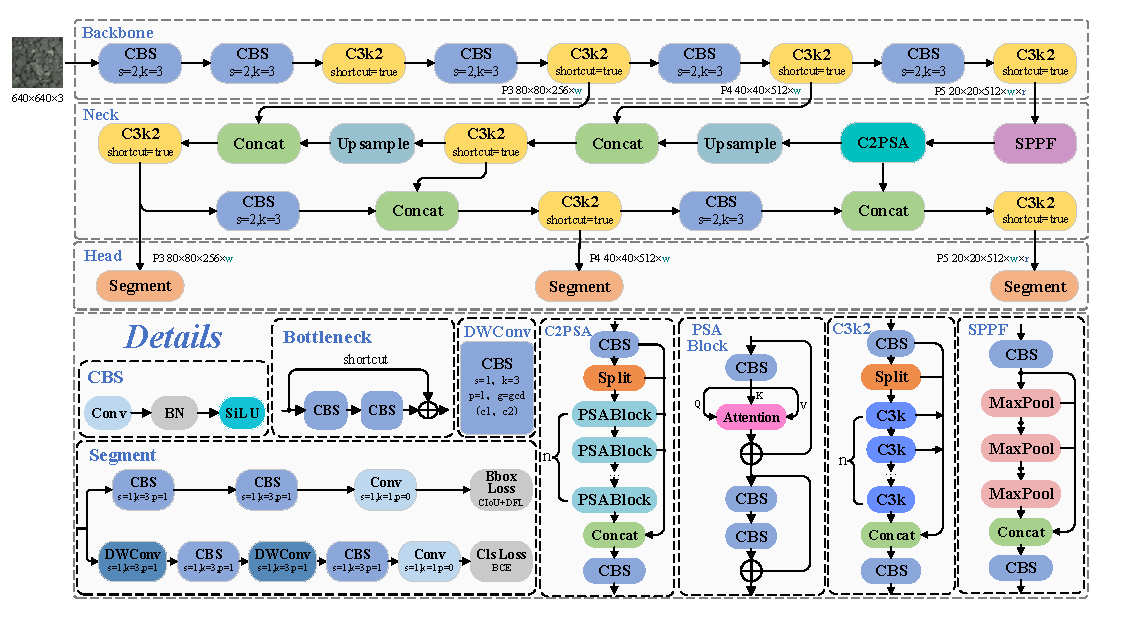
\includegraphics[width=\textwidth]{figures/yolo11-seg-architecture}
    \caption{Arsitektur YOLO11-seg}
    \label{fig:arsitektur-yolo11-seg}
    \par\smallskip
    {\footnotesize Sumber: \cite{qiu2025}}
\end{figure}

\noindent\textbf{\textit{Backbone}.}
Pada bagian paling kiri diagram, citra masukan diproses secara bertahap melalui rangkaian modul CBS dan C3k2. CBS terdiri atas operasi konvolusi, \textit{batch normalization}, dan fungsi aktivasi SiLU, sedangkan C3k2 digunakan untuk melanjutkan proses ekstraksi fitur secara efisien. Setelah melewati beberapa tahapan tersebut, fitur diproses oleh SPPF (\textit{Spatial Pyramid Pooling--Fast}) untuk mengumpulkan informasi konteks melalui operasi \textit{pooling} pada beberapa cakupan. Bagian akhir \textit{backbone} memuat modul C2PSA yang menggunakan mekanisme perhatian untuk menekankan informasi fitur yang relevan. Susunan pada diagram juga menunjukkan bahwa ukuran spasial fitur semakin mengecil pada tahapan yang lebih dalam, sementara informasi yang dibawa fitur menjadi semakin kaya \cite{khanam2024,qiu2025}.

% Aktifkan blok berikut setelah gambar close-up backbone tersedia.
% Jika gambar dipotong dari diagram asli, gunakan keterangan ``Diadaptasi dari''.
% \begin{figure}[H]
%     \centering
%     \includegraphics[width=0.9\textwidth]{figures/yolo11-seg-backbone}
%     \caption{Bagian \textit{backbone} pada arsitektur YOLO11-seg}
%     \label{fig:backbone-yolo11-seg}
%     \par\smallskip
%     {\footnotesize Sumber: Diadaptasi dari \cite{qiu2025}}
% \end{figure}

\noindent\textbf{\textit{Neck}.}
Bagian tengah diagram memperlihatkan bahwa fitur dari beberapa tingkat \textit{backbone} tidak langsung diteruskan ke keluaran. Fitur tersebut terlebih dahulu diproses melalui operasi \textit{upsample}, \textit{concat}, CBS, dan C3k2. Operasi \textit{upsample} memperbesar resolusi peta fitur, sedangkan \textit{concat} menggabungkan fitur tersebut dengan fitur dari tahapan lain. Jalur penggabungan berlangsung dari fitur yang lebih dalam menuju fitur beresolusi lebih tinggi dan kemudian kembali menuju fitur beresolusi lebih rendah. Dengan susunan tersebut, \textit{neck} memadukan detail spasial dari fitur beresolusi tinggi dengan informasi semantik dari fitur yang lebih dalam. Hasilnya adalah tiga tingkat fitur, yaitu P3, P4, dan P5, yang diteruskan ke bagian keluaran \cite{khanam2024,qiu2025}.

% Aktifkan blok berikut setelah gambar close-up neck tersedia.
% \begin{figure}[H]
%     \centering
%     \includegraphics[width=0.9\textwidth]{figures/yolo11-seg-neck}
%     \caption{Penggabungan fitur pada bagian \textit{neck} YOLO11-seg}
%     \label{fig:neck-yolo11-seg}
%     \par\smallskip
%     {\footnotesize Sumber: Diadaptasi dari \cite{qiu2025}}
% \end{figure}

\noindent\textbf{\textit{Segmentation head}.}
Pada bagian kanan diagram, fitur P3, P4, dan P5 masing-masing terhubung dengan satu blok \textit{Segment}. Ketiga tingkat fitur tersebut memungkinkan model melakukan prediksi terhadap objek dengan ukuran yang berbeda. Setiap blok \textit{Segment} menghasilkan informasi yang diperlukan untuk memprediksi kelas objek, posisi \textit{bounding box}, dan segmentasi instans. Dengan demikian, klasifikasi lauk, penentuan lokasi objek, dan segmentasi tidak dilakukan oleh tiga model yang terpisah, tetapi dihasilkan dari fitur bersama dalam satu arsitektur YOLO11-seg \cite{qiu2025}.

% Aktifkan blok berikut setelah gambar close-up segmentation head tersedia.
% \begin{figure}[H]
%     \centering
%     \includegraphics[width=0.9\textwidth]{figures/yolo11-seg-head}
%     \caption{Bagian \textit{segmentation head} pada arsitektur YOLO11-seg}
%     \label{fig:head-yolo11-seg}
%     \par\smallskip
%     {\footnotesize Sumber: Diadaptasi dari \cite{qiu2025}}
% \end{figure}

Mekanisme pembentukan \textit{mask} pada bagian keluaran mengikuti konsep dua cabang. Cabang pertama menghasilkan prediksi kelas, koordinat \textit{bounding box}, dan koefisien \textit{mask} untuk setiap kandidat objek. Cabang kedua menghasilkan sekumpulan \textit{prototype mask} yang digunakan bersama. Koefisien \textit{mask} dari suatu objek kemudian dikombinasikan dengan \textit{prototype mask} untuk membentuk \textit{mask} khusus bagi instans tersebut. Oleh karena itu, dua objek dengan kelas yang sama tetap dapat memperoleh \textit{mask} yang berbeda dan dihitung sebagai dua instans terpisah \cite{qiu2025}.

% Diagram utama tidak memperlihatkan proses pembentukan mask secara terperinci.
% Gambar berikut sebaiknya dibuat ulang sebagai diagram sederhana yang menunjukkan
% alur prototype mask + koefisien mask -> mask setiap instans.
% \begin{figure}[H]
%     \centering
%     \includegraphics[width=0.8\textwidth]{figures/yolo11-seg-mask-formation}
%     \caption{Mekanisme pembentukan \textit{mask} setiap instans pada YOLO11-seg}
%     \label{fig:pembentukan-mask-yolo11-seg}
%     \par\smallskip
%     {\footnotesize Sumber: Diadaptasi dari \cite{qiu2025}}
% \end{figure}

Melalui alur tersebut, satu citra dapat menghasilkan sejumlah prediksi instans yang masing-masing memiliki kelas, lokasi, dan \textit{mask}. Dalam penelitian ini, kelas hasil prediksi digunakan untuk menentukan jenis lauk, sedangkan jumlah instans pada setiap kelas digunakan dalam proses kalkulasi harga.

\subsubsection*{b. Pelatihan YOLO11-seg}

Pelatihan model dapat dimulai dari bobot pralatih agar fitur visual yang telah dipelajari sebelumnya dapat digunakan sebagai titik awal dan kemudian disesuaikan dengan kelas pada dataset penelitian. Pada penelitian ini, bobot YOLO11-seg disesuaikan untuk mengenali sembilan kelas, yaitu nasi, rendang, ayam goreng, perkedel, sayur nangka, daun singkong, telur dadar, telur kari, dan sambal.

Pada proses pelatihan, citra dan \textit{ground truth} diberikan kepada model untuk menghasilkan prediksi lokasi objek, kelas, dan segmentasi. Prediksi tersebut dibandingkan dengan \textit{ground truth} untuk memperoleh nilai \textit{loss}. Nilai \textit{loss} kemudian digunakan dalam proses \textit{backpropagation} untuk memperbarui bobot model secara berulang. Data validasi digunakan untuk memantau performa model selama pelatihan, sedangkan data pengujian digunakan setelah model akhir diperoleh.

Nilai parameter pelatihan, seperti varian YOLO11-seg, ukuran citra masukan, jumlah \textit{epoch}, \textit{batch size}, konfigurasi augmentasi, dan parameter lain yang digunakan pada implementasi dijelaskan pada Bab III.

\input{chapters/subchapters/2/2-3-4}
\input{chapters/subchapters/2/2-3-5}
\input{chapters/subchapters/2/2-3-6}


\chapter{RANCANGAN DAN PEMBUATAN}

\section{Rancangan Sistem}

Sistem yang dirancang merupakan sistem \textit{checkout} otomatis untuk mengenali dan menghitung lauk Nasi Padang menggunakan YOLO11-seg. Sistem dirancang sebagai \textit{proof-of-concept} mekanisme \textit{self-service} bagi pelanggan \textit{dine-in}, di mana pelanggan dapat mengambil lauk secara mandiri kemudian meletakkan piring pada area pengambilan citra untuk dilakukan proses \textit{checkout}.

Pada sistem ini, kamera ditempatkan pada posisi tetap di atas area pengambilan citra untuk memperoleh citra piring yang berisi lauk pilihan pelanggan. Citra tersebut kemudian diproses menggunakan model YOLO11-seg yang telah dilatih untuk mengenali sembilan kelas, yaitu nasi, rendang, ayam goreng, perkedel, sayur nangka, daun singkong, telur dadar, telur kari, dan sambal. Model menghasilkan prediksi kelas dan \textit{segmentation mask} untuk setiap instans lauk yang dikenali.

Sebelum dapat digunakan pada proses \textit{checkout}, model YOLO11-seg terlebih dahulu melalui tahap pelatihan. Tahap tersebut dimulai dari pengumpulan citra Nasi Padang, anotasi setiap instans lauk, pembagian dataset, serta augmentasi pada data pelatihan. Dataset yang telah disiapkan kemudian digunakan untuk melatih YOLO11-seg sehingga model dapat mempelajari karakteristik visual dari masing-masing kelas lauk.

Setelah proses pelatihan selesai, model yang diperoleh digunakan pada tahap inferensi. Pada tahap ini, setiap hasil prediksi diperlakukan sebagai satu instans lauk dan dikelompokkan berdasarkan kelasnya. Jumlah instans pada setiap kelas kemudian digunakan oleh program kalkulasi harga. Program mencocokkan kelas lauk dengan harga tetap yang telah ditentukan dan menghitung total harga berdasarkan jumlah instans yang dikenali.

Perancangan sistem dilakukan melalui beberapa tahap yang mencakup perencanaan sistem, analisis kebutuhan sistem, dan perancangan alur sistem secara lebih rinci. Perencanaan sistem membahas tahapan yang diperlukan mulai dari persiapan dataset hingga model dapat digunakan pada proses \textit{checkout}. Analisis sistem membahas kebutuhan yang diperlukan dalam pengembangan sistem, sedangkan perancangan sistem membahas alur pelatihan, inferensi, penghitungan instans, dan kalkulasi harga.

\subsection{Perencanaan Sistem}

Perencanaan sistem \textit{checkout} otomatis Nasi Padang dilakukan melalui beberapa tahap yang dimulai dari persiapan data hingga model dapat digunakan dalam proses \textit{checkout}. Tahap awal dilakukan dengan mengumpulkan citra Nasi Padang yang memuat objek dari kelas yang akan dikenali. Citra yang telah dikumpulkan kemudian diperiksa dan dipilih agar dapat digunakan sebagai dataset dalam penelitian.

Setiap citra yang digunakan pada proses pelatihan selanjutnya diberikan anotasi untuk menunjukkan kelas dan area dari setiap instans lauk. Anotasi dibuat dalam bentuk \textit{segmentation mask} sehingga setiap objek pada citra memiliki informasi kelas dan batas objek yang digunakan sebagai \textit{ground truth} pada proses pelatihan YOLO11-seg.

Dataset yang telah dianotasi kemudian dibagi menjadi data pelatihan, validasi, dan pengujian. Pembagian dilakukan sebelum proses augmentasi agar citra hasil augmentasi tidak tersebar pada bagian dataset yang berbeda. Augmentasi hanya diterapkan pada data pelatihan untuk menambah variasi citra yang digunakan selama proses pembelajaran model \cite{yang2022augmentation,tampu2022}.

Data pelatihan selanjutnya digunakan untuk melatih YOLO11-seg. Pada proses pelatihan, model menerima citra beserta \textit{ground truth} dan menghasilkan prediksi lokasi objek, kelas, serta \textit{segmentation mask}. Hasil prediksi dibandingkan dengan \textit{ground truth} untuk memperoleh nilai \textit{loss}, kemudian bobot model diperbarui melalui proses \textit{backpropagation}. Proses tersebut dilakukan secara berulang hingga diperoleh model akhir yang digunakan pada tahap inferensi.

Pada tahap inferensi, citra piring yang diperoleh dari kamera diberikan kepada model yang telah dilatih. Model menghasilkan sejumlah instans objek yang masing-masing memiliki informasi kelas dan \textit{segmentation mask}. Setiap instans yang dikenali kemudian dihitung berdasarkan kelasnya sehingga diperoleh jumlah lauk dari masing-masing kelas.

Hasil penghitungan tersebut selanjutnya diteruskan ke program kalkulasi harga. Program mencocokkan setiap kelas lauk dengan harga tetap yang telah ditentukan, kemudian menghitung subtotal berdasarkan jumlah instans pada kelas tersebut. Seluruh subtotal dijumlahkan untuk menghasilkan total harga yang harus dibayarkan pada proses \textit{checkout}.

Tahap persiapan dataset yang digunakan dalam perencanaan sistem dijelaskan lebih lanjut pada subbagian berikut.

\input{chapters/subchapters/3/3-1-1-1}
\input{chapters/subchapters/3/3-1-1-2}
\input{chapters/subchapters/3/3-1-1-3}
\input{chapters/subchapters/3/3-1-1-4}

\subsection{Analisis Sistem}

Tahap analisis sistem dilakukan untuk menentukan kebutuhan yang diperlukan dalam pengembangan sistem \textit{checkout} otomatis Nasi Padang. Analisis mencakup kebutuhan perangkat keras, perangkat lunak, data, dan fungsi yang harus dijalankan oleh sistem.

Perangkat keras yang diperlukan meliputi:
\begin{enumerate}
    \item kamera untuk memperoleh citra piring dari posisi tetap di atas area pengambilan citra;
    \item perangkat komputasi untuk melakukan anotasi data, pelatihan, validasi, pengujian, dan inferensi YOLO11-seg;
    \item media penyimpanan untuk menyimpan citra, anotasi, bobot model, serta hasil pengujian; dan
    \item area pengambilan citra yang memungkinkan posisi kamera dipertahankan tetap dengan kondisi pencahayaan yang relatif konsisten.
\end{enumerate}

Perangkat lunak yang diperlukan meliputi:
\begin{enumerate}
    \item Python sebagai bahasa pemrograman utama untuk pengolahan data, pelatihan model, dan pengembangan program;
    \item Ultralytics sebagai \textit{framework} yang digunakan untuk pelatihan, validasi, pengujian, dan inferensi YOLO11-seg;
    \item CVAT sebagai perangkat anotasi kelas dan poligon untuk setiap instans objek makanan; dan
    \item pustaka pendukung yang diperlukan untuk pengolahan citra, pengelolaan dataset, serta implementasi program kalkulasi harga.
\end{enumerate}

Data utama yang dibutuhkan berupa citra Nasi Padang beserta anotasi poligon dan label kelas untuk setiap instans. Sistem juga memerlukan tabel harga tetap yang memuat pasangan antara kelas makanan dan harga satuan.

Secara fungsional, sistem harus mampu menerima citra dari kamera, menghasilkan prediksi kelas dan \textit{segmentation mask} untuk setiap instans, menghitung jumlah instans berdasarkan kelas, mencocokkan hasil tersebut dengan tabel harga, serta menghitung subtotal dan total harga. Spesifikasi perangkat dan versi perangkat lunak yang benar-benar digunakan dicatat pada tahap pembuatan sistem.

\subsection{Perancangan Sistem}

Tahap perancangan sistem bertujuan menggambarkan alur kerja sistem \textit{checkout} otomatis Nasi Padang mulai dari pelatihan model hingga penggunaan model pada proses \textit{checkout}. Perancangan dibagi menjadi dua bagian, yaitu rancangan pelatihan model YOLO11-seg dan rancangan proses \textit{checkout}.

Rancangan pelatihan model menjelaskan alur penggunaan dataset yang telah dianotasi dan dibagi menjadi data pelatihan, validasi, dan pengujian. Data pelatihan digunakan untuk melatih YOLO11-seg melalui proses prediksi, perhitungan \textit{loss}, dan pembaruan bobot model. Performa model dipantau menggunakan data validasi hingga diperoleh model akhir yang digunakan dalam proses pengujian dan inferensi.

Rancangan proses \textit{checkout} menjelaskan alur pengolahan citra piring yang diperoleh dari kamera. Model YOLO11-seg menghasilkan prediksi kelas dan \textit{segmentation mask} untuk setiap instans objek makanan. Setiap instans kemudian dihitung berdasarkan kelasnya dan dicocokkan dengan tabel harga tetap untuk memperoleh subtotal setiap kelas serta total harga keseluruhan.

Rancangan pelatihan model dan proses \textit{checkout} dijelaskan lebih lanjut pada subbagian berikut.

\input{chapters/subchapters/3/3-1-3-1}
\input{chapters/subchapters/3/3-1-3-2}


\section{Pembuatan Sistem}

Tahap pembuatan sistem merupakan penerapan rancangan yang telah dijelaskan pada bagian sebelumnya menjadi sistem \textit{checkout} otomatis Nasi Padang. Pembuatan mencakup penyelesaian dataset, pelatihan dan evaluasi YOLO11-seg, serta implementasi program \textit{checkout} yang mengolah hasil inferensi menjadi jumlah instans dan total harga.

Pada tahap penyelesaian dataset, citra yang telah lolos proses seleksi dianotasi berdasarkan sembilan kelas penelitian, kemudian dibagi menjadi data pelatihan, validasi, dan pengujian. Augmentasi diterapkan melalui \textit{pipeline} pelatihan pada data pelatihan.

Model YOLO11-seg dilatih menggunakan dataset yang telah disiapkan dengan bobot pralatih sebagai titik awal. Bobot model dipantau menggunakan data validasi, sedangkan model terpilih dievaluasi menggunakan data pengujian sebelum digunakan pada proses \textit{checkout}.

Program \textit{checkout} menerima hasil inferensi model, menghitung jumlah instans berdasarkan kelas, mencocokkan setiap kelas dengan tabel harga tetap, serta menghitung subtotal dan total harga. Spesifikasi perangkat keras, perangkat lunak, konfigurasi pelatihan, hasil pembuatan dataset, dan detail implementasi program akan dicatat berdasarkan pelaksanaan sistem yang sebenarnya sehingga tidak ditetapkan sebelum proses implementasi dilakukan.



% =========================================================
% REFERENCES — BibTeX
% =========================================================
\clearpage
\bibliographystyle{IEEEtran}
\bibliography{references}

\end{document}
